\documentclass[11pt,a4paper]{article}

\usepackage[T1]{fontenc}
\usepackage[utf8]{inputenc}
\usepackage{lmodern}
\usepackage{microtype}
\usepackage[margin=2.3cm]{geometry}
\usepackage{amsmath,amssymb,amsthm,mathtools}
\usepackage{booktabs,tabularx,multirow}
\usepackage{xcolor}
\usepackage{tikz}
\usetikzlibrary{arrows.meta,positioning,calc}
\usepackage{pgfplots}
\pgfplotsset{compat=1.17}
\usepackage{caption,subcaption}
\usepackage{enumitem}
\usepackage{listings}
\usepackage{float}
\usepackage[colorlinks=true,linkcolor=blue!50!black,citecolor=blue!50!black,urlcolor=blue!50!black]{hyperref}
\usepackage{cleveref}

\setlist{itemsep=2pt,topsep=4pt}
\setlength{\emergencystretch}{3em}
\captionsetup{font=small,labelfont=bf}

\newcommand{\att}{\rightharpoonup}
\newcommand{\odd}{\hookrightarrow}
\newcommand{\AF}{\mathit{AF}}
\newcommand{\Mgr}{M^{\mathit{grnd}}_{\AF}}
\newcommand{\EGR}{E_{\mathit{GR}}}
\newcommand{\code}[1]{{\let\origus\_\renewcommand{\_}{\origus\allowbreak}\texttt{#1}}}

\definecolor{inC}{HTML}{86EFAC}
\definecolor{outC}{HTML}{FCA5A5}
\definecolor{undecC}{HTML}{FDE68A}
\definecolor{agx}{HTML}{2563EB}
\definecolor{agy}{HTML}{9333EA}
\definecolor{agz}{HTML}{EA580C}

\tikzset{
  arg/.style={circle,draw=black!70,line width=0.6pt,minimum size=8.5mm,inner sep=0pt,font=\small},
  ain/.style={arg,fill=inC},
  aout/.style={arg,fill=outC},
  aundec/.style={arg,fill=undecC},
  hid/.style={arg,draw=black!40,dashed,text=black!40},
  ox/.style={draw=agx,line width=1.6pt},
  oy/.style={draw=agy,line width=1.6pt},
  oz/.style={draw=agz,line width=1.6pt},
  atk/.style={-{Stealth[length=2.6mm]},line width=0.7pt,black!65},
  hot/.style={-{Stealth[length=2.6mm]},line width=1.4pt,red!75!black},
}

\lstset{basicstyle=\ttfamily\small,columns=fullflexible,frame=single,framerule=0.3pt,
  rulecolor=\color{black!25},backgroundcolor=\color{black!3},xleftmargin=4pt,xrightmargin=4pt}

\theoremstyle{definition}
\newtheorem*{thm53}{Theorem 5.3 (Rahwan)}
\newtheorem*{thm54}{Theorem 5.4 (Rahwan)}

\title{\textbf{Argumentation among Agents:\\ Dung Semantics and Strategyproof Argumentation Mechanisms}\\[4pt]
\large CSL7650 Autonomous Systems \,·\, Assignment 3}
\author{% TODO: replace with the team's names and roll numbers
  [Name 1, Roll No.] \qquad [Name 2, Roll No.]}
\date{November 2026}

\begin{document}
\maketitle

\begin{abstract}
We implement an engine for abstract argumentation frameworks (conflict-freeness, defence, the
characteristic function, and the grounded, complete, preferred, stable and semi-stable semantics,
legal labellings and acceptance status) and the strategic layer of Chapter~5 of Weiss'
\emph{Multiagent Systems}: the grounded direct argumentation mechanism, exhaustive best responses,
an exact test of the strategyproofness characterisation (Theorem~5.3), and a cycle-safe test of the
graph-theoretic sufficient condition (Theorem~5.4). Every example in the chapter is reproduced by
39 automated tests. On $3\times1000$ random three-agent frameworks the mechanism is strategyproof in
57.8\,\%, 27.5\,\% and 14.7\,\% of instances for attack probabilities $p=0.15,0.25,0.35$. No instance
satisfies Theorem~5.4's condition without being strategyproof, including in a targeted stress test of
3000 condition-satisfying instances. Of the 956 instances that are strategyproof although the
condition fails, we explain every one by one of four structural reasons. We also show that random
self-attacks, which the brief's generator allows, dominate the Theorem~5.4 statistics, and report a
second run without them.
\end{abstract}

\section{Introduction}

Abstract argumentation \cite{dung1995} models a debate as a directed graph whose nodes are arguments
and whose edges are attacks. A semantics selects the sets of arguments that can be accepted together.
When the arguments come from self-interested agents, a further question arises: will an agent reveal
all its arguments, or can it gain by withholding some? Chapter~5 of \cite{weiss2013} (by Rahwan)
studies this with \emph{argumentation mechanism design}: agents report subsets of their arguments,
the mechanism accepts the grounded extension of everything reported, and each agent wants as many of
its own arguments accepted as possible.

The assignment has three parts: (i) an engine for Dung's semantics, (ii) functions for the strategic
setting, and (iii) experiments on random frameworks that test Theorem~5.4 and probe its limits. This
report describes the design (\cref{sec:impl}), validates it against the textbook
(\cref{sec:validation}), and answers the three experimental questions (\cref{sec:setup,sec:results}).
\Cref{sec:discussion} discusses modelling choices that affect the numbers, and \cref{sec:demo}
describes the interactive demonstration.

\section{Background}\label{sec:background}

An \emph{argumentation framework} is a pair $\AF=\langle A,\att\rangle$ with $\att\subseteq A\times A$.
For $S\subseteq A$ let $S^+=\{\beta : \exists\alpha\in S,\ \alpha\att\beta\}$ and
$\alpha^-=\{\beta:\beta\att\alpha\}$. Following Definitions~5.2--5.7 of the chapter:
\begin{itemize}
  \item $S$ is \emph{conflict-free} if $S\cap S^+=\emptyset$; $S$ \emph{defends} $\alpha$ if
        $\alpha^-\subseteq S^+$.
  \item The \emph{characteristic function} is $\mathcal F(S)=\{\alpha : S \text{ defends } \alpha\}$.
  \item $S$ is \emph{admissible} if it is conflict-free and $S\subseteq\mathcal F(S)$, and
        \emph{complete} if it is conflict-free and $S=\mathcal F(S)$.
  \item The \emph{grounded} extension is the least fixed point of $\mathcal F$; \emph{preferred}
        extensions are the $\subseteq$-maximal complete extensions; a \emph{stable} extension is
        conflict-free with $S^+=A\setminus S$; \emph{semi-stable} extensions are complete extensions
        with $\subseteq$-maximal range $S\cup S^+$.
  \item A \emph{legal labelling} maps each argument to \textsf{in}, \textsf{out} or \textsf{undec}
        such that an argument is \textsf{in} iff all its attackers are \textsf{out}, and \textsf{out}
        iff some attacker is \textsf{in} (Definition~5.6). The \textsf{in}-sets of legal labellings
        are exactly the complete extensions.
  \item Under a semantics with extensions $\mathcal E$, an argument is \emph{skeptically accepted}
        if it is in every extension, \emph{credulously accepted} if it is in at least one, and
        \emph{rejected} otherwise (Definition~5.8).
\end{itemize}

\paragraph{Strategic setting.} Each agent $i$ privately holds a set of arguments $A_i$ (its
\emph{type}) and reports some $A_i^\circ\subseteq A_i$; agents may hide arguments but cannot invent
them. The \emph{grounded direct argumentation mechanism} $\Mgr$ (Definition~5.21) outputs
$\EGR\bigl(\langle A_1^\circ\cup\dots\cup A_I^\circ,\ \att\rangle\bigr)$, the grounded extension of the
framework induced by the reported arguments. Agents have \emph{acceptability-maximising} preferences
(Definition~5.22); we use $u_i(o)=|A_i\cap o|$, counted against the \emph{true} type.

\begin{thm53}
$\Mgr$ is strategyproof for agents with acceptability-maximising preferences iff for every agent
$i$, every $S\subseteq A_i$ and every report profile $A_{-i}$ of the others,
$|A_i\cap\EGR(\langle A_i\cup A_{-i},\att\rangle)| \ge |A_i\cap\EGR(\langle (A_i\setminus S)\cup
A_{-i},\att\rangle)|$.
\end{thm53}

Write $\alpha\odd\beta$ (``$\alpha$ indirectly defeats $\beta$'') if there is an odd-length path from
$\alpha$ to $\beta$ in the whole argument graph.

\begin{thm54}
If no agent $i$ has $\alpha_1,\alpha_2\in A_i$ with $\alpha_1\odd\alpha_2$, then $\Mgr$ is
strategyproof.
\end{thm54}

Theorem~5.3 is an exact characterisation but needs exponential enumeration. Theorem~5.4 is a cheap
graph test but only \emph{sufficient}: Example~5.11 is strategyproof although the condition fails.

\section{Implementation}\label{sec:impl}

The code is plain Python~3 with no dependencies (the demonstration additionally uses Streamlit).
\Cref{tab:modules} lists the modules.

\begin{table}[H]
\centering\small
\begin{tabularx}{\textwidth}{@{}lX@{}}
\toprule
Module & Contents \\
\midrule
\code{argumentation.py} & \code{ArgumentationFramework}: all of Part~1. \\
\code{strategic.py} & Mechanism, best responses, Theorem~5.3 and Theorem~5.4 checks. \\
\code{analysis.py} & Classifier that explains why an instance is strategyproof although Theorem~5.4's condition fails (Q3). \\
\code{experiments.py} & Random generator, the main experiment, the no-self-attack run and the stress test. \\
\code{tests/} & 39 unit tests, mostly textbook examples (\cref{sec:validation}). \\
\code{app.py}, \code{ui.py} & Interactive demonstration (\cref{sec:demo}). \\
\bottomrule
\end{tabularx}
\caption{Code organisation.}\label{tab:modules}
\end{table}

\subsection{Argumentation engine}

\code{ArgumentationFramework(arguments, attacks)} validates its input and precomputes, for every
argument, its attackers $\alpha^-$ and the arguments it attacks. Frameworks are immutable, so derived
results can be shared safely. The assignment's functions map directly onto methods:

\begin{itemize}
  \item \code{is\_conflict\_free(S)} checks $S^+\cap S=\emptyset$; \code{defends(S, a)} checks
        $\alpha^-\subseteq S^+$; \code{characteristic\_function(S)} returns
        $\{\alpha : \alpha^-\subseteq S^+\}$ in a single pass.
  \item \code{is\_admissible} and \code{is\_complete} combine these tests exactly as in the
        definitions.
  \item \textbf{(A)} \code{grounded\_extension()} iterates $\emptyset,\mathcal F(\emptyset),
        \mathcal F^2(\emptyset),\dots$ until the set stops changing. Because $\mathcal F$ is monotone
        and $A$ is finite, this reaches the least fixed point in at most $|A|+1$ steps.
  \item \textbf{(B)} \code{complete\_extensions()} enumerates all $2^{|A|}$ subsets in increasing size
        and keeps those that are conflict-free fixed points of $\mathcal F$.
  \item \textbf{(C)} \code{preferred\_extensions()} keeps the inclusion-maximal complete extensions;
        \code{stable\_extensions()} tests every conflict-free subset for $S^+=A\setminus S$;
        \code{semi\_stable\_extensions()} keeps the complete extensions whose range $S\cup S^+$ is
        inclusion-maximal.
  \item \textbf{(D)} \code{legal\_labellings()} enumerates all $3^{|A|}$ total labellings and keeps
        those satisfying the two conditions of Definition~5.6 for every argument.
  \item \textbf{(E)} \code{acceptance\_status(a, semantics)} returns whether $\alpha$ is skeptically
        accepted, credulously accepted or rejected. If the semantics has no extensions (possible
        only for stable semantics) it raises \code{NoExtensionsError} rather than returning a
        vacuous answer.
\end{itemize}

Enumeration is exponential, which is unavoidable for preferred, stable and semi-stable reasoning in
general and harmless for the $\le 8$-argument frameworks of the assignment: a full analysis of one
8-argument framework takes well under a second.

\subsection{Strategic functions}

\paragraph{(1) Mechanism.} \code{grounded\_direct\_argumentation\_mechanism(af, reports)} takes the
union of the reported sets, builds the induced subframework (only attacks between reported
arguments survive) and returns its grounded extension.

\paragraph{(2) Best responses.} \code{best\_responses(af, types, i, others)} fixes the other agents'
reports, evaluates the mechanism for each of the $2^{|A_i|}$ subsets agent $i$ could reveal, and
returns every report attaining the maximum utility, together with the full table of utilities and
outcomes (used by the demonstration).

\paragraph{(3) Theorem~5.3.} \code{check\_theorem\_5\_3(af, types)} implements the characterisation
literally. For each agent $i$ and each combination of the other agents' subsets, it compares the
truthful utility with the utility of every subset $A_i\setminus S$; ties count in favour of truth.
For three agents this is $\sum_i 2^{|A_i|}\prod_{j\ne i}2^{|A_j|}=3\cdot2^{|A|}$ comparisons, at most
768 for eight arguments. Since an outcome depends only on the \emph{union} of the reports, grounded
extensions are cached per union, so at most $2^{|A|}$ of them are computed. The function returns the
first profitable deviation it finds, which the demonstration replays.

\paragraph{(4) Theorem~5.4.} The condition fails iff some agent owns $\alpha,\beta$ (possibly equal)
with an odd-length path $\alpha\odd\beta$. Searching for odd paths naively loops forever on cyclic
graphs. We instead run a breadth-first search over \emph{states} $(\text{argument},\
\text{parity of the length so far})$, starting from $(\alpha,0)$ and looking for $(\beta,1)$:
\begin{lstlisting}
queue <- [(alpha, 0)];  seen <- {(alpha, 0)}
while queue not empty:
    (v, q) <- pop front;   if (v, q) = (beta, 1): reconstruct path and stop
    for every w with v attacks w:  if (w, 1-q) not in seen: add it and push it
\end{lstlisting}
There are only $2|A|$ states, so the search always terminates, in $O(|A|+|{\att}|)$ time per pair, and
it naturally handles cycles: an odd cycle simply moves the search into the opposite parity. The
witness it reconstructs is an odd \emph{walk}, which may repeat vertices. We also implemented the
stricter reading, an odd \emph{simple} path (\code{find\_odd\_simple\_path}, a depth-first search
that never revisits a vertex). Both readings agree on every instance we generated
(\cref{sec:discussion}). Pairs with $\alpha=\beta$ are included, so an owned self-attacking argument
or an odd cycle through an owned argument violates the condition, matching the theorem's requirement
that each type be conflict-free ``explicitly and implicitly''. \code{odd\_path\_witnesses} returns
every violating pair, not just the first.

\subsection{Explaining condition failures (Q3)}

For an instance that is strategyproof although the condition fails, \code{explain\_condition\_failure}
labels every violating pair $(\alpha,\beta)$ of each agent with the first applicable reason:
\begin{enumerate}[label=(\alph*)]
  \item $\beta$ attacks itself, so grounded semantics never accepts it;
  \item $\beta$ is in no grounded extension of any induced subframework (it is ``dead'');
  \item $\alpha=\beta$, i.e.\ the path is an odd cycle back to the same argument;
  \item $\alpha\att\beta$ directly (an explicit conflict inside the type);
  \item otherwise, a live indirect odd path of length at least three.
\end{enumerate}
The instance is then assigned the most demanding reason present, in the order
(e)\,$>$\,(d)\,$>$\,(c)\,$>$\,(b)\,$>$\,(a). For example, an instance with both a direct conflict and
an indirect path is classified by the indirect path, since that is the harder case to explain.

\section{Validation against the textbook}\label{sec:validation}

The brief asks us to test the functions on the book's examples. \Cref{tab:book} summarises the checks
encoded in \code{tests/test\_book\_examples.py}; another file, \code{tests/test\_strategic.py}, covers
odd-path edge cases (self-loops, even and odd cycles, unreachable targets, the walk and simple-path
readings) and the reproducibility of the random generator. All 39 tests pass
(\code{python -m unittest discover -s tests -t .}).

\begin{table}[H]
\centering\small
\begin{tabularx}{\textwidth}{@{}lX@{}}
\toprule
Source & Checked (all reproduced) \\
\midrule
Fig.~5.1 & $\{\alpha_3,\alpha_5\}$ defends $\alpha_1$. Admissible sets (Ex.~5.5) are $\emptyset$,
  $\{\alpha_3\}$, $\{\alpha_5\}$, $\{\alpha_3,\alpha_5\}$, $\{\alpha_1,\alpha_3,\alpha_5\}$.
  $\{\alpha_3,\alpha_5\}$ is not complete; $\mathcal F(\{\alpha_3\})=\{\alpha_3,\alpha_5\}$ (Ex.~5.6).
  The iteration gives $\mathcal F^1(\emptyset)=\{\alpha_3,\alpha_5\}$,
  $\mathcal F^2(\emptyset)=\{\alpha_1,\alpha_3,\alpha_5\}$. Grounded = unique complete = preferred =
  stable = $\{\alpha_1,\alpha_3,\alpha_5\}$; exactly one legal labelling. \\
Fig.~5.2 & Complete extensions $\{\alpha_3\}$, $\{\alpha_1,\alpha_3\}$, $\{\alpha_2,\alpha_3\}$
  (Ex.~5.7); grounded $\{\alpha_3\}$; preferred = stable = semi-stable =
  $\{\alpha_1,\alpha_3\},\{\alpha_2,\alpha_3\}$ (Ex.~5.8); three legal labellings (the three panels of
  the figure). $\alpha_1$ is credulously but not skeptically accepted under preferred semantics and
  rejected under grounded; $\alpha_3$ is skeptically accepted everywhere. \\
Fig.~5.3 & Grounded extension $\{a,c,e\}$, the outcome of the dispute tree of Ex.~5.9. \\
Ex.~5.10 & Truthful outcome $\{\alpha_1,\alpha_3\}$ with $u_x=1$, $u_y=0$, $u_z=1$; if $x$ hides
  $\alpha_1$ the outcome is $\{\alpha_2,\alpha_4,\alpha_5\}$ and $u_x=2$; $x$'s unique best response is
  $\{\alpha_4,\alpha_5\}$; the Theorem~5.3 check reports ``not strategyproof''; Theorem~5.4 witness
  $\alpha_1\to\alpha_2\to\alpha_3\to\alpha_4$. \\
Ex.~5.11 & Truthful outcome $\{\alpha_1,\alpha_4,\alpha_5,\alpha_6\}$; strategyproof by the
  Theorem~5.3 check although the Theorem~5.4 condition fails; the classifier puts it in the
  ``neutralised indirect path'' category. \\
\bottomrule
\end{tabularx}
\caption{Textbook examples reproduced by the test suite.}\label{tab:book}
\end{table}

\paragraph{Misprints.} As the brief anticipates, two statements in the chapter are wrong and our
results show the corrections:
\begin{enumerate}
  \item \textbf{Example~5.10} prints $u_y(o,\{\alpha_3\})=1$ and $u_z(o,\{\alpha_2\})=0$, attaching
        each utility to the other agent's arguments. Since $A_y=\{\alpha_2\}$, $A_z=\{\alpha_3\}$ and
        $o=\{\alpha_1,\alpha_3\}$, the correct values are $u_y=0$ and $u_z=1$.
  \item \textbf{After Example~5.11} the text says that $\alpha_5$ removes $x$'s incentive to hide
        $\alpha_1$. It is $\alpha_6$, the new argument that defeats $\alpha_3$
        (\cref{fig:ex511}): with $\alpha_6$ revealed, $\alpha_3$ is \textsf{out} whatever $x$ does
        with $\alpha_1$, so $\alpha_4,\alpha_5$ are accepted anyway and hiding $\alpha_1$ only loses
        it.
\end{enumerate}

\begin{figure}[H]
\centering
\begin{subfigure}{0.48\textwidth}\centering
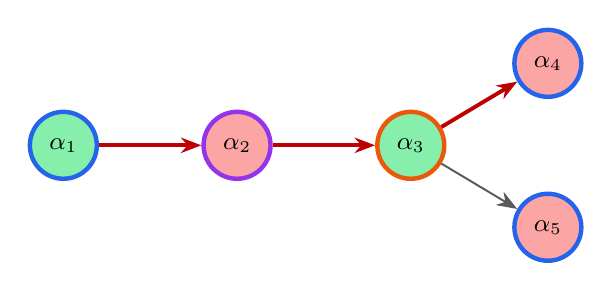
\begin{tikzpicture}[node distance=13mm]
  \node[ain,ox] (a1) {$\alpha_1$};
  \node[aout,oy,right=of a1] (a2) {$\alpha_2$};
  \node[ain,oz,right=of a2] (a3) {$\alpha_3$};
  \node[aout,ox,above right=4mm and 11mm of a3] (a4) {$\alpha_4$};
  \node[aout,ox,below right=4mm and 11mm of a3] (a5) {$\alpha_5$};
  \draw[hot] (a1)--(a2); \draw[hot] (a2)--(a3); \draw[hot] (a3)--(a4); \draw[atk] (a3)--(a5);
\end{tikzpicture}
\caption{Ex.~5.10, truthful: $o=\{\alpha_1,\alpha_3\}$, $u_x=1$.}
\end{subfigure}\hfill
\begin{subfigure}{0.48\textwidth}\centering
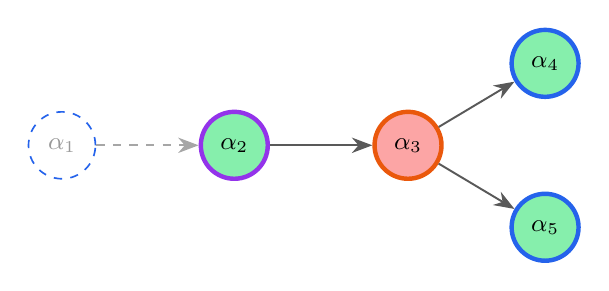
\begin{tikzpicture}[node distance=13mm]
  \node[hid,draw=agx] (a1) {$\alpha_1$};
  \node[ain,oy,right=of a1] (a2) {$\alpha_2$};
  \node[aout,oz,right=of a2] (a3) {$\alpha_3$};
  \node[ain,ox,above right=4mm and 11mm of a3] (a4) {$\alpha_4$};
  \node[ain,ox,below right=4mm and 11mm of a3] (a5) {$\alpha_5$};
  \draw[atk,dashed,black!35] (a1)--(a2); \draw[atk] (a2)--(a3); \draw[atk] (a3)--(a4); \draw[atk] (a3)--(a5);
\end{tikzpicture}
\caption{$x$ hides $\alpha_1$: $o=\{\alpha_2,\alpha_4,\alpha_5\}$, $u_x=2$.}
\end{subfigure}

\vspace{4mm}
\begin{subfigure}{0.6\textwidth}\centering
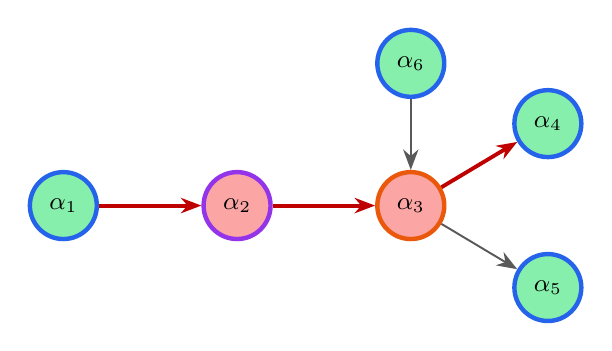
\begin{tikzpicture}[node distance=13mm]
  \node[ain,ox] (a1) {$\alpha_1$};
  \node[aout,oy,right=of a1] (a2) {$\alpha_2$};
  \node[aout,oz,right=of a2] (a3) {$\alpha_3$};
  \node[ain,ox,above right=4mm and 11mm of a3] (a4) {$\alpha_4$};
  \node[ain,ox,below right=4mm and 11mm of a3] (a5) {$\alpha_5$};
  \node[ain,ox,above=9mm of a3] (a6) {$\alpha_6$};
  \draw[hot] (a1)--(a2); \draw[hot] (a2)--(a3); \draw[hot] (a3)--(a4); \draw[atk] (a3)--(a5);
  \draw[atk] (a6)--(a3);
\end{tikzpicture}
\caption{Ex.~5.11: $\alpha_6$ defeats $\alpha_3$; truth is a best response although
$\alpha_1\odd\alpha_4$.}\label{fig:ex511}
\end{subfigure}
\caption{Examples~5.10 and~5.11 with their grounded labellings (green \textsf{in}, red \textsf{out}).
Border colour marks the owner: \textcolor{agx}{$x$}, \textcolor{agy}{$y$}, \textcolor{agz}{$z$}.
The bold red chain is the Theorem~5.4 witness found by our search.}\label{fig:ex510}
\end{figure}

\section{Experimental setup}\label{sec:setup}

\paragraph{Generator.} Following the brief, each instance has three agents $x,y,z$ and
$n\in\{6,7,8\}$ arguments, with $n$ drawn uniformly. Each ordered pair $(\alpha,\beta)$ is an attack
independently with probability $p\in\{0.15,0.25,0.35\}$. Each argument is assigned to an agent
uniformly at random, conditioned on every agent owning at least one argument. We generate 1000
instances per value of $p$.

\paragraph{Self-attacks.} ``Each possible attack'' includes the $n$ self-pairs $(\alpha,\alpha)$, so
the default run samples them like any other pair. This matters a great deal for Theorem~5.4: every
argument is owned by someone, so a single self-attack anywhere is an owned odd path of length one and
falsifies the condition. Between 69\,\% and 96\,\% of default instances contain a self-attack
(\cref{tab:q1}). We therefore also report a second run with self-attacks excluded. Each instance seed
draws the same random numbers in both runs, so the two runs contain the same graphs except for the
self-loops, and differences between them are attributable to self-attacks alone.

\paragraph{Measurements.} For every instance we record whether the mechanism is strategyproof
(exact Theorem~5.3 check), whether Theorem~5.4's condition holds (walk and simple-path readings), and,
when the condition fails but the mechanism is strategyproof, the Q3 category. Proportions are reported
with 95\,\% Wilson score intervals \cite{wilson1927}.

\paragraph{Stress test for Q2.} Because the condition rarely holds in the main run, we also sample
instances (no self-attacks, $p$ drawn uniformly from the three values) until 3000 instances satisfying
the condition have been collected, and test each for strategyproofness.

\paragraph{Reproducibility.} Everything is seeded (master seed 2026). The three commands
\code{python experiments.py}, \code{python experiments.py --no-self-attacks} and
\code{python experiments.py --stress 3000} regenerate every number in this report in under a minute,
writing summaries, per-instance CSV files and the interesting cases to \code{results/}.

\section{Results}\label{sec:results}

\subsection*{Q1: How often is the mechanism strategyproof?}

\begin{table}[H]
\centering\small
\begin{tabular}{@{}l c c c c c c@{}}
\toprule
& \multicolumn{4}{c}{With self-attacks (default)} & \multicolumn{2}{c}{Without self-attacks} \\
\cmidrule(lr){2-5}\cmidrule(l){6-7}
$p$ & SP & 95\,\% CI & Cond.\ holds & Self-attack inst. & SP & Cond.\ holds \\
\midrule
0.15 & 578 (57.8\,\%) & 54.7--60.8\,\% & 39 & 689 & 641 (64.1\,\%) & 138 \\
0.25 & 275 (27.5\,\%) & 24.8--30.3\,\% & 5  & 859 & 320 (32.0\,\%) & 33 \\
0.35 & 147 (14.7\,\%) & 12.6--17.0\,\% & 0  & 955 & 114 (11.4\,\%) & 4 \\
\midrule
Total & 1000 / 3000 & & 44 & 2503 & 1075 / 3000 & 175 \\
\bottomrule
\end{tabular}
\caption{Strategyproof (SP) instances and instances satisfying Theorem~5.4's condition, out of 1000
per value of $p$. Without self-attacks the 95\,\% intervals are 61.1--67.0\,\%, 29.2--35.0\,\% and
9.6--13.5\,\%.}\label{tab:q1}
\end{table}

\begin{figure}[H]
\centering
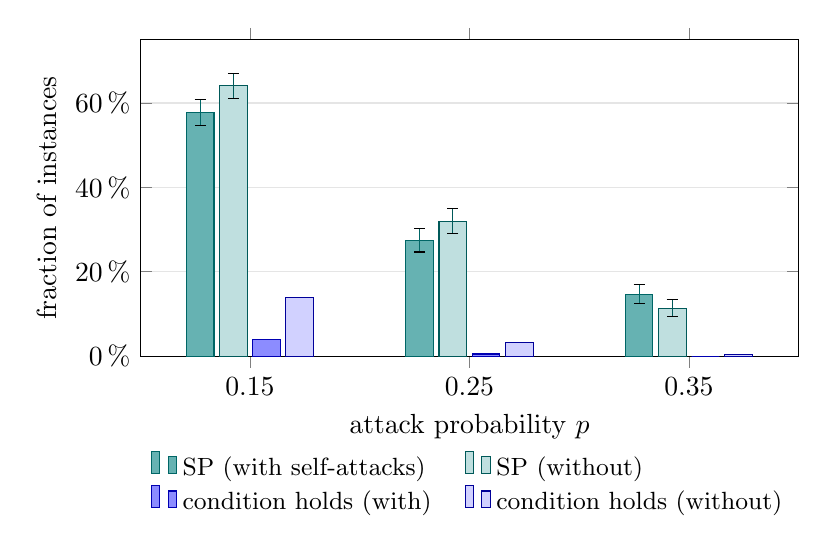
\begin{tikzpicture}
\begin{axis}[
  ybar, bar width=10pt, width=0.82\textwidth, height=5.6cm,
  ymin=0, ymax=0.75, ylabel={fraction of instances},
  yticklabel={\pgfmathparse{\tick*100}\pgfmathprintnumber{\pgfmathresult}\,\%},
  symbolic x coords={0.15,0.25,0.35}, xtick=data, xlabel={attack probability $p$},
  enlarge x limits=0.25, legend style={at={(0.5,-0.28)},anchor=north,font=\small,draw=none,legend columns=2,/tikz/every even column/.append style={column sep=1em}},
  legend cell align=left, ymajorgrids, grid style={black!10},
  every node near coord/.append style={font=\scriptsize},
  error bars/y dir=both, error bars/y explicit,
]
\addplot[fill=teal!60,draw=teal!80!black] coordinates {
  (0.15,0.578) +- (0,0.031) (0.25,0.275) +- (0,0.028) (0.35,0.147) +- (0,0.022)};
\addplot[fill=teal!25,draw=teal!70!black] coordinates {
  (0.15,0.641) +- (0,0.030) (0.25,0.320) +- (0,0.029) (0.35,0.114) +- (0,0.020)};
\addplot[fill=blue!45,draw=blue!70!black,error bars/.cd,y dir=none] coordinates {
  (0.15,0.039) (0.25,0.005) (0.35,0.0)};
\addplot[fill=blue!18,draw=blue!60!black,error bars/.cd,y dir=none] coordinates {
  (0.15,0.138) (0.25,0.033) (0.35,0.004)};
\legend{SP (with self-attacks), SP (without), condition holds (with), condition holds (without)}
\end{axis}
\end{tikzpicture}
\caption{Strategyproofness and Theorem~5.4's condition against attack density, with approximate
95\,\% intervals on the strategyproof fractions.}\label{fig:q1}
\end{figure}

Strategyproofness falls steeply with density: from 57.8\,\% at $p=0.15$ to 14.7\,\% at $p=0.35$
(64.1\,\% to 11.4\,\% without self-attacks). The intervals are narrow and do not overlap, so the trend
is not noise. The explanation is structural. With more attacks, each agent is more likely to own two
arguments joined by an odd chain through other agents' arguments, which is exactly the pattern of
Example~5.10, where hiding the head of the chain re-instates arguments further down. Theorem~5.4's
condition collapses even faster (3.9\,\%, 0.5\,\%, 0\,\% with self-attacks), because it forbids
\emph{every} such chain, whether or not it can be exploited.

\subsection*{Q2: Does the condition ever hold without strategyproofness?}

\textbf{No.} In the default run all 44 condition-satisfying instances are strategyproof; without
self-attacks all 175 are. The simple-path reading of ``odd path'' selects exactly the same instances,
so the conclusion does not depend on the reading. Since 44 is a small sample, the stress test
examined 53\,955 random instances to collect 3000 that satisfy the condition (2401, 520 and 79 at
$p=0.15,0.25,0.35$). \textbf{All 3000 are strategyproof.} This is consistent with Theorem~5.4 being a
correct sufficient condition, which the book proves; a single counterexample would have indicated a
bug in our implementation or an error in the theorem.

The intuition behind the theorem is visible in the data. If every directed path between two of an
agent's arguments has even length, then each of its arguments can only act as an (indirect)
\emph{defender} of its other arguments, never as an (indirect) attacker. Withholding an argument can
then only remove defence, so it can never raise the number of the agent's arguments in the grounded
extension.

\subsection*{Q3: Strategyproof although the condition fails --- why?}

956 default instances (900 without self-attacks) are strategyproof although the condition fails. The
classifier assigns each one to one of the categories in \cref{tab:q3}; no instance needed the
``dead victim'' category, and no instance was left unexplained.

\begin{table}[H]
\centering\small
\begin{tabularx}{\textwidth}{@{}X r r r r r@{}}
\toprule
& \multicolumn{4}{c}{With self-attacks} & Without \\
\cmidrule(lr){2-5}\cmidrule(l){6-6}
Category (most demanding reason present) & 0.15 & 0.25 & 0.35 & Total & Total \\
\midrule
Live indirect odd path, neutralised (Ex.~5.11 type) & 166 & 150 & 107 & 423 & 396 \\
Only direct conflicts between own arguments & 261 & 64 & 19 & 344 & 503 \\
Only odd cycles back to the same argument & 8 & 11 & 13 & 32 & 1 \\
Every odd path ends at a self-attacking argument & 104 & 45 & 8 & 157 & 0 \\
\midrule
Total & 539 & 270 & 147 & 956 & 900 \\
\bottomrule
\end{tabularx}
\caption{Why the mechanism is strategyproof although Theorem~5.4's condition fails.}\label{tab:q3}
\end{table}

Each category has a concrete reason why the odd path never translates into a profitable lie. All four
examples below are from the generated data and can be opened in the demonstration.

\paragraph{Self-attacking victims (157).} If every odd path of an agent ends at an argument that
attacks itself, nothing is at stake: grounded semantics never accepts a self-attacking argument, so
revealing the path's source cannot cost the agent anything. In \code{p15\_0019}, $y$ owns
$\{a_1,a_4,a_5\}$; $a_1$ attacks itself and is also attacked by $a_4$ and $a_5$. All three violating
pairs end at $a_1$, which is never accepted. These instances are artefacts of self-attacks and vanish
in the second run.

\paragraph{Direct conflicts only (344; 503 without self-attacks).} Here the only violations are
single attacks $\alpha\att\beta$ inside a type. Hiding $\alpha$ may free $\beta$, but $\alpha$ is then
lost, so the trade is at best one-for-one, and a tie does not make lying profitable. In
\code{p15\_0001}, $x$ owns $\{a_1,a_2,a_6\}$ with $a_6\att a_1$. Truthfully $x$ gets $\{a_6\}$; hiding
$a_6$ gives $\{a_1\}$: one argument either way. A direct conflict becomes exploitable only if $\beta$
in turn defends further arguments of the same agent, which then makes a longer indirect path the
binding reason.

\paragraph{Odd cycles only (32; 1 without self-attacks).} An odd cycle $\alpha\to\dots\to\alpha$
through other agents' arguments makes $\alpha$ indirectly attack itself. Hiding $\alpha$ removes
$\alpha$ itself, so it cannot increase $\alpha$'s own acceptance. In this category $\alpha$ has no odd
path to any \emph{other} live argument of its owner (that would put the instance in a higher
category), so hiding $\alpha$ cannot rescue anything else either. In \code{p25\_0187} (no
self-attacks, \cref{fig:q3}a), $x$ owns $a_1$ on the cycle $a_1\to a_6\to a_4\to a_1$. When everything
is revealed the three cycle arguments are \textsf{undec}; if $y$ or $z$ withhold part of the cycle,
$a_1$ may become \textsf{in} or \textsf{out}, but $x$'s other argument $a_3$ is unattacked and never
depends on $a_1$. So for every report of the others, hiding $a_1$ can only lose $a_1$.

\paragraph{Neutralised indirect path (423; 396 without self-attacks).} These are genuine
Example~5.11 situations: an agent owns $\alpha\odd\beta$ through a chain of length at least three, but
the chain cannot be exploited, either because another argument already defends $\beta$ or because
breaking the chain costs exactly as much as it gains. In \code{p15\_0402} (\cref{fig:q3}b), $z$ owns
$a_1,a_5,a_7$ with $a_1\to a_2\to a_4\to a_7$. Agent $x$'s argument $a_6$ also attacks $a_4$, exactly
like $\alpha_6$ in Example~5.11. Truthfully $z$ gets $\{a_1,a_5,a_7\}$ (utility 3); hiding $a_1$
re-instates $a_2$ but $a_4$ stays \textsf{out} because of $a_6$, so $z$ only loses $a_1$. Even when
$x$ withholds $a_6$, hiding $a_1$ merely ties with truth ($\{a_5,a_7\}$ versus $\{a_1,a_5\}$).

\begin{figure}[H]
\centering
\begin{subfigure}{0.42\textwidth}\centering
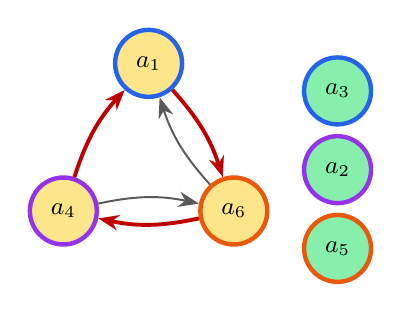
\begin{tikzpicture}
  \node[aundec,ox] (a1) at (90:1.25) {$a_1$};
  \node[aundec,oz] (a6) at (330:1.25) {$a_6$};
  \node[aundec,oy] (a4) at (210:1.25) {$a_4$};
  \draw[hot] (a1) to[bend left=12] (a6);
  \draw[hot] (a6) to[bend left=12] (a4);
  \draw[hot] (a4) to[bend left=12] (a1);
  \draw[atk] (a6) to[bend left=12] (a1);
  \draw[atk] (a4) to[bend left=12] (a6);
  \node[ain,ox] at (2.4,0.9) {$a_3$};
  \node[ain,oy] at (2.4,-0.1) {$a_2$};
  \node[ain,oz] at (2.4,-1.1) {$a_5$};
\end{tikzpicture}
\caption{\code{p25\_0187}: odd cycle through $x$'s $a_1$.}
\end{subfigure}\hfill
\begin{subfigure}{0.55\textwidth}\centering
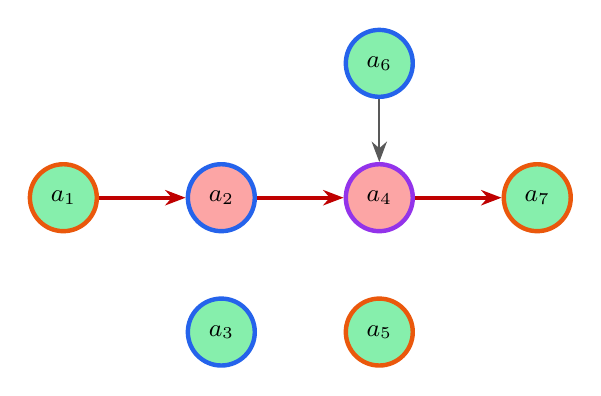
\begin{tikzpicture}[node distance=11mm]
  \node[ain,oz] (a1) {$a_1$};
  \node[aout,ox,right=of a1] (a2) {$a_2$};
  \node[aout,oy,right=of a2] (a4) {$a_4$};
  \node[ain,oz,right=of a4] (a7) {$a_7$};
  \node[ain,ox,above=8mm of a4] (a6) {$a_6$};
  \node[ain,ox,below=8mm of a2] (a3) {$a_3$};
  \node[ain,oz,below=8mm of a4] (a5) {$a_5$};
  \draw[hot] (a1)--(a2); \draw[hot] (a2)--(a4); \draw[hot] (a4)--(a7);
  \draw[atk] (a6)--(a4);
\end{tikzpicture}
\caption{\code{p15\_0402}: $a_6$ shields $a_7$ as in Ex.~5.11.}
\end{subfigure}
\caption{Two Q3 instances with their grounded labellings (yellow = \textsf{undec}). The odd path that
falsifies Theorem~5.4 is drawn in bold red.}\label{fig:q3}
\end{figure}

The common thread is that Theorem~5.4 looks only at the graph between an agent's own arguments,
whereas strategyproofness also depends on what \emph{other} arguments do to the path (defenders such as
$a_6$, self-attacks, undecided cycles) and on the arithmetic of what is gained versus lost. The
condition is therefore sufficient but far from necessary: in the default run only 44 of the 1000
strategyproof instances satisfy it.

\section{Discussion}\label{sec:discussion}

\paragraph{The effect of self-attacks.} Self-attacks make the condition fail in 2503 of 3000 default
instances, so the default ``condition holds'' fraction mostly measures how often the generator draws a
self-loop. Their effect on strategyproofness is subtler and changes sign with density
(\cref{tab:q1}: removing them raises SP at $p=0.15$ and $0.25$ but lowers it at $p=0.35$). Comparing
the two runs instance by instance reveals two opposing mechanisms:
\begin{itemize}
  \item \emph{Self-attacks create lies.} 225 instances are strategyproof only without self-attacks. In
        200 of them the profitable lie hides a self-attacking argument. Such an argument is never
        accepted, so it contributes no utility to its owner, yet it still attacks the owner's other
        arguments; hiding it is free.
  \item \emph{Self-attacks prevent lies.} 150 instances are strategyproof only \emph{with}
        self-attacks. In 143 of them, the argument the liar would gain in the self-attack-free graph
        is itself self-attacking (so it is never accepted) or is attacked by a self-attacking
        argument, which keeps it out of the grounded extension unless something else defeats the
        self-attacker. Either way the gain disappears and the lie no longer pays.
\end{itemize}
The second effect grows with the number of self-loops, i.e.\ with $p$ (29, 45 and 76 instances),
while the first does not (92, 90, 43), which explains the crossover.

\paragraph{Reading of ``odd-length path''.} The book defines $\alpha\odd\beta$ by an odd-length path.
We use odd walks (vertices may repeat), which the parity search finds efficiently and which handles
cycles cleanly, and we include $\alpha=\beta$. Odd walks and odd simple paths gave the same verdict on
all 9000 generated instances (both runs and the stress test), so this choice does not affect any
number. Including $\alpha=\beta$ does matter: dropping it would change the verdict on three
self-attack-free instances, each with an odd cycle through an agent's own argument (e.g.\
\code{p25\_0187}). All three are strategyproof, so Q2 is unaffected either way. We keep $\alpha=\beta$
because the theorem asks for each type to be conflict-free, and an owned self-attacking argument
violates that.

\paragraph{Limitations.} The engine and both theorem checks are exhaustive, so they are exponential in
the number of arguments; this is fine up to roughly 12--15 arguments but would need SAT- or
labelling-based algorithms for larger frameworks. The experiments fix three agents, uniform
ownership and the counting utility $|A_i\cap o|$; other preference classes from the chapter (for
example, focal-argument preferences) can make the mechanism manipulable in different ways. Finally,
agents may only hide arguments, as in the chapter; allowing invented arguments would change the
problem entirely.

\section{Demonstration}\label{sec:demo}

The demonstration is an interactive Streamlit application (\code{streamlit run app.py}) that calls the
same tested modules, so it cannot disagree with the reported results. It has four tabs:
\begin{itemize}
  \item \textbf{Semantics:} any textbook figure, random instance, experiment case or custom framework
        is drawn and coloured by its grounded labelling or any legal labelling. The tab shows the
        $\mathcal F^k(\emptyset)$ iteration, all extensions, the labellings tagged with the semantics
        they match, the acceptance status of every argument, and a tester for conflict-free,
        admissible and complete sets.
  \item \textbf{Strategic mechanism:} the user toggles each agent's reports and sees the outcome and
        utilities update live; the Theorem~5.3 check can replay its counterexample (e.g.\ $x$ hiding
        $\alpha_1$ in Example~5.10), the Theorem~5.4 witness is highlighted on the graph, and a table
        lists every report an agent could make with its utility.
  \item \textbf{Experiments:} the Q1 chart for both runs, the Q2 counts and stress test, and the Q3
        categories with a browser that loads any instance into the mechanism tab.
  \item \textbf{Notes:} the two misprints and the modelling choices above.
\end{itemize}

\section{Conclusion}

We implemented and validated every function the assignment asks for; all textbook examples are
reproduced, and the two misprints are corrected. Experimentally, the grounded direct mechanism is
strategyproof for a majority of sparse random frameworks but for only about one in seven dense ones.
Theorem~5.4's condition was never satisfied by a manipulable instance, even among 3000 instances
selected to satisfy it, but it is far from necessary: most strategyproof instances violate it, for
four identifiable reasons, the most interesting being the Example~5.11 pattern in which a third
argument shields the end of an agent's own odd chain. Finally, whether random generators allow
self-attacks changes the Theorem~5.4 statistics completely and shifts strategyproofness in both
directions, so it should always be stated.

\begin{thebibliography}{9}
\bibitem{weiss2013} G.~Weiss (ed.). \emph{Multiagent Systems}, 2nd ed. MIT Press, 2013.
  Chapter~5: I.~Rahwan, ``Argumentation among Agents''.
\bibitem{dung1995} P.~M.~Dung. On the acceptability of arguments and its fundamental role in
  nonmonotonic reasoning, logic programming and $n$-person games. \emph{Artificial Intelligence},
  77(2):321--357, 1995.
\bibitem{rahwan2008} I.~Rahwan and K.~Larson. Mechanism design for abstract argumentation. In
  \emph{Proc.\ AAMAS}, pages 1031--1038, 2008.
\bibitem{caminada2006} M.~Caminada. On the issue of reinstatement in argumentation. In \emph{Proc.\
  JELIA}, LNCS 4160, pages 111--123, 2006.
\bibitem{wilson1927} E.~B.~Wilson. Probable inference, the law of succession, and statistical
  inference. \emph{Journal of the American Statistical Association}, 22(158):209--212, 1927.
\end{thebibliography}

\end{document}
